\title[Causality]{Causality: Lecture 11}
\author[Joris Mooij]{\\[5mm]\large Joris Mooij \& Patrick Forr\'e\\
\url{j.m.mooij@uva.nl}, \url{p.d.forre@uva.nl}}
\institute[UvA]{University of Amsterdam}
\date[2022-04-19]{\normalsize April 19th, 2023}
\maketitle

\part{$\sigma$-Separation and Acyclifications}
\frame{\partpage}

\begin{frame}{(Un)blockable non-colliders}
Remember: $\Sc^G(v) := \Anc^G(v) \cap \Desc^G(v)$.
\begin{Def}[\ref{def:unblockable_noncollider}]
  Let $G=(J,V,E,L)$ be a CDMG and $ \pi =\lp  v_0 \sus \cdots \sus v_n \rp $ a walk in $G$.
  We call a non-collider $v_k$ on $\pi$ an \emph{unblockable non-collider} on $\pi$ if it is not an end-node ($k \notin \{0,n\}$) and it only has outgoing edges on $\pi$ to nodes in the same strongly connected component of $G$. That is,
  it is one of the following patterns:
  \[\begin{array}{rccl}
    v_{k-1} \hut v_k \hus v_{k+1} & \text{ with } & v_{k-1} \in \Sc^G(v_{k})\\
    v_{k-1} \suh v_k \tuh v_{k+1} & \text{ with } & v_{k+1} \in \Sc^G(v_{k})\\
    v_{k-1} \hut v_k \tuh v_{k+1} & \text{ with } & v_{k-1} \in \Sc^G(v_k) \land v_{k+1} \in \Sc^G(v_k)
  \end{array}\]
  Otherwise, $v_k$ is called a \emph{blockable non-collider} on $\pi$.
  This means that $v_k$ is either an end-node ($k \in \lC 0,n\rC$) or it has at least one outgoing arrow 
  $v_k \tuh v_{k\pm1}$ pointing to a node $v_{k\pm1}$ that lies in a different strongly connected component than $v_k$, i.e.\ $v_{k\pm1} \notin \Sc^G(v_k)$.
\end{Def}
\end{frame}

\begin{frame}{Running example}
  \begin{Eg}
  \centering
  \begin{tikzpicture}
    \begin{scope}
      \node[ndint] (X1) at (0,0) {$X_1$};
      \node[ndout] (X2) at (1.5,0) {$X_2$};
      \node[ndout] (X3) at (3,0) {$X_3$};
      \node[ndout] (X4) at (0,-1.5) {$X_4$};
      \node[ndout] (X5) at (3,-1.5) {$X_5$};
      \node[ndout] (X6) at (1.5,-2.5) {$X_6$};
      \node[ndint] (X7) at (-1.5,-1.5) {$X_7$};
      \node[ndout] (X8) at (0,-3) {$X_8$};
      \draw[arint] (X1) -- (X4);
      \draw[arout] (X2) -- (X4);
      \draw[arout] (X2) -- (X3);
      \draw[arout] (X3) -- (X5);
      \draw[arout] (X4) -- (X5);
      \draw[arout] (X5) -- (X6);
      \draw[arout] (X6) -- (X4);
      \draw[arint] (X4) -- (X8);
      \draw[arout] (X7) -- (X8);
    \end{scope}
  \end{tikzpicture}
  \begin{itemize}
    \item Give an example of a walk with an unblockable noncollider;
    \item Give an example of a walk with an blockable noncollider.
  \end{itemize}
  \end{Eg}
\end{frame}

\begin{frame}{$\sigma$-blocked walks}
\begin{Def}[\ref{def:sigma_blocking}]
  Let $G=(J,V,E,L)$ be a CDMG and $ \pi =\lp  v_0 \sus \cdots \sus v_n \rp $ a walk in $G$,
  and $C \ins J \cup V$ a subset of nodes.
  We say that the walk $\pi$ is:
    \emph{$C$-$\sigma$-open} (or \emph{$\sigma$-open given $C$}) if and only if:
  \begin{enumerate}
      \item all colliders $v_k$ on $\pi$ are in $\Anc^G(C)$, \emph{and}:
    \item all blockable non-colliders $v_k$ on $\pi$ are \emph{not} in $C$.
      % all of its adjacent children, $v_{k\pm 1}$, on $\pi$ lie in its strongly connected component $\Sc^G(v_k)$. \Joris{the last part ``all of its neighboring children on $\pi$ lie in its strongly connected component'' is equivalent to ``unblockable'' (see Definition~\ref{def:unblockable_noncollider}); we might move that definition to here for convenience.}
  \end{enumerate}
  Otherwise, we say that the walk $\pi$ is
  \emph{$C$-$\sigma$-blocked}  (or \emph{$\sigma$-blocked given $C$}), that is:
  \begin{enumerate}
    \item there exists a collider $v_k$ on $\pi$ that is \emph{not} in $\Anc^G(C)$, \emph{or}:
    \item there exists a blockable non-collider $v_k$ on $\pi$ in $C$.
  \end{enumerate}  
  Note that unblockable non-colliders are always $C$-$\sigma$-open, regardless of the subset $C \ins V \cup J$.
\end{Def}
If $G$ is acyclic then all non-colliders are blockable, and then $\pi$ is $C$-$\sigma$-open iff $\pi$ is $C$-$d$-open.
\end{frame}

\begin{frame}{Running example}
  \begin{Eg}
  \centering
  \begin{tikzpicture}
    \begin{scope}
      \node[ndint] (X1) at (0,0) {$X_1$};
      \node[ndout] (X2) at (1.5,0) {$X_2$};
      \node[ndout] (X3) at (3,0) {$X_3$};
      \node[ndout] (X4) at (0,-1.5) {$X_4$};
      \node[ndout] (X5) at (3,-1.5) {$X_5$};
      \node[ndout] (X6) at (1.5,-2.5) {$X_6$};
      \node[ndint] (X7) at (-1.5,-1.5) {$X_7$};
      \node[ndout] (X8) at (0,-3) {$X_8$};
      \draw[arint] (X1) -- (X4);
      \draw[arout] (X2) -- (X4);
      \draw[arout] (X2) -- (X3);
      \draw[arout] (X3) -- (X5);
      \draw[arout] (X4) -- (X5);
      \draw[arout] (X5) -- (X6);
      \draw[arout] (X6) -- (X4);
      \draw[arint] (X4) -- (X8);
      \draw[arout] (X7) -- (X8);
    \end{scope}
  \end{tikzpicture}
  \begin{itemize}
    \item Give an example of a walk that is $\sigma$-blocked given $X_4$;
    \item Give an example of a walk that is $\sigma$-open given $X_4$;
  \end{itemize}
  \end{Eg}
\end{frame}

%\frame{\frametitle{$\sigma$-Blocking and $\sigma$-Separation}
%\begin{definition}
%  Let $G = \lt J,E,V,L \rt$ be a CDMG and $C \subseteq J \cup V$ a subset of nodes and $\pi$ a walk in $G$:
%  $$\pi = v_0 \sus \dots \sus v_n.$$
%  $\pi$ is called \emph{$C$-$\sigma$-blocked}, or \emph{$\sigma$-blocked by $C$}, iff
%  \begin{itemize}
%    \item $v_0 \in C$ or $v_n \in C$, or
%    \item it contains a collider $v_{k-1} \suh v_k \hus v_{k+1}$ with $v_k \not\in \Anc^G(C)$, or
%    \item it contains a non-collider
%      $v_{k-1} \sus v_k \tuh v_{k+1}$  with $v_k \in C$
%    \alert{and such that $v_{k+1} \notin \Sc^{G}(v_k)$}, or
%    \item it contains a non-collider
%      $v_{k-1} \hut v_k \sus v_{k+1}$ with $v_k \in C$
%    \alert{and such that $v_{k-1} \notin \Sc^{G}(v_k)$}.
%  \end{itemize}
%  We say that \emph{$A$ is $\sigma$-separated from $B$ by $C$}, denoted \emph{$A \Perp^{\alert{\sigma}}_G B \mid C$}, if every walk with one end node in $A$ and one end node in $B \cup J$ is $\sigma$-blocked by $C$.
%\end{definition}
%}

\begin{frame}{$\sigma$-Blocking and $\sigma$-Separation}
\begin{Def}[\ref{def:sigma_separation}]
    Let $G=(J,V,E,L)$ be a CDMG and $A,B,C \ins J \cup V$ (not necessarily disjoint) subset of nodes.
    We then say that:
    \begin{enumerate}
        \item \emph{$A$ is $\sigma$-separated from $B$ given $C$ in $G$}, in symbols:
    \[ A \Perp^\sigma_G B \given C, \]
      if every walk from a node in $A$ to a node in $B \alert{\cup J}$ is $C$-$\sigma$-blocked by $C$.
        \item If that property does not hold we will write:
            \[ A \nPerp^\sigma_G B \given C. \]
        \item We also define the special case:
                \[ A \Perp^\sigma_G B \qquad :\iff \qquad A \Perp^\sigma_GB \given \emptyset.\]
    \end{enumerate}
\end{Def}
\end{frame}

\begin{frame}{Running example}
  \begin{Eg}
  \centering
  \begin{tikzpicture}
    \begin{scope}
      \node[ndint] (X1) at (0,0) {$X_1$};
      \node[ndout] (X2) at (1.5,0) {$X_2$};
      \node[ndout] (X3) at (3,0) {$X_3$};
      \node[ndout] (X4) at (0,-1.5) {$X_4$};
      \node[ndout] (X5) at (3,-1.5) {$X_5$};
      \node[ndout] (X6) at (1.5,-2.5) {$X_6$};
      \node[ndint] (X7) at (-1.5,-1.5) {$X_7$};
      \node[ndout] (X8) at (0,-3) {$X_8$};
      \draw[arint] (X1) -- (X4);
      \draw[arout] (X2) -- (X4);
      \draw[arout] (X2) -- (X3);
      \draw[arout] (X3) -- (X5);
      \draw[arout] (X4) -- (X5);
      \draw[arout] (X5) -- (X6);
      \draw[arout] (X6) -- (X4);
      \draw[arint] (X4) -- (X8);
      \draw[arout] (X7) -- (X8);
    \end{scope}
  \end{tikzpicture}
  \begin{itemize}
    \item Give an example of a $\sigma$-separation given $X_4$;
    \item Give an example of a $\sigma$-connection given $X_4$.
  \end{itemize}
  \end{Eg}
\end{frame}

\frame{\frametitle{Example: $\sigma$-Separation}
\begin{example}
  \begin{tikzpicture}
      \node at (1,3.5) {Graph $G(M)$:};
      \node[ndout] (X1) at (0,0) {$X_1$};
      \node[ndout] (X2) at (1.5,0) {$X_2$};
      \node[ndout] (X3) at (1.5,1.5) {$X_3$};
      \node[ndout] (X4) at (0,1.5) {$X_4$};
      \node[ndlat] (W1) at (-1,-1) {$W_1$};
      \node[ndlat] (W2) at (2.5,-1) {$W_2$};
      \node[ndlat] (W3) at (2.5,2.5) {$W_3$};
      \node[ndlat] (W4) at (-1,2.5) {$W_4$};
      \draw[arout] (X1) edge (X2);
      \draw[arout] (X2) edge (X3);
      \draw[arout] (X3) edge (X4);
      \draw[arout] (X4) edge (X1);
      \draw[arout] (W1) edge (X1);
      \draw[arout] (W2) edge (X2);
      \draw[arout] (W3) edge (X3);
      \draw[arout] (W4) edge (X4);
      \node at (-3,3.5) {SCM $M$:};
      \node[text width=4cm] at (-3,1) {\small $X_1=X_4+W_1$\\
      $X_2=X_1 \cdot W_2$\\
      $X_3=X_2+W_3$\\
      $X_4=X_3\cdot W_4$\\
      \,\\
      $W_1,W_2,W_3,W_4$\\ independent};
      \node at (5,1.75) {is $X_1 \displaystyle\Perp^d X_3 \given X_2, X_4$?};
%      \node at (5,1) {but};
      \node at (5,0.25) {is $X_1 \displaystyle\Perp^\sigma X_3 \given X_2, X_4$?};
  \end{tikzpicture}
\end{example}

\bigskip
In general: No $\sigma$-separations between nodes within the same strongly connected component (for any separation set).
}

\begin{frame}{Graphical Acyclifications: Definition}
\begin{Def}[\ref{def:cdg_acyclification}]
  Given a CDMG $G = ( J, V, E, L)$, we call a CADMG $G' = (J, V, E', L')$
  an \emph{acyclification of $G$} if
  \begin{enumerate}
    \item $G'$ is acyclic;
    \item $G'$ has the same input nodes $J$ and output nodes $V$ as $G$;
    \item for every pair of nodes $(i,j)$ such that $i \not\in\Sc^G(j)$:
      \begin{enumerate}
      \item $i \tuh j \in E'$ iff there exists a node $j' \in \Sc^G(j)$ such that $i \tuh j' \in E$;
      \item $i \huh j \in L'$ iff there exist nodes $i' \in \Sc^G(i), j' \in \Sc^G(j)$ such that $i' \huh j' \in L$;
      \end{enumerate}
  \item for every pair of distinct nodes $(i,j)$ such that $i \in\Sc^G(j)$: $i \tuh j \in E'$ or $i \hut j \in E'$ or $i \huh j \in L'$.
  \end{enumerate}
\end{Def}
\end{frame}

\begin{frame}{Graphical Acyclifications: Example}
  \centering
  \scalebox{0.8}{\begin{tikzpicture}
    \begin{scope}
      \node at (0.75,1) {CDMG $G$:};
      \node[ndint] (X1) at (0,0) {$X_1$};
      \node[ndout] (X2) at (1.5,0) {$X_2$};
      \node[ndout] (X3) at (3,0) {$X_3$};
      \node[ndout] (X4) at (0,-1.5) {$X_4$};
      \node[ndout] (X5) at (3,-1.5) {$X_5$};
      \node[ndout] (X6) at (1.5,-2.5) {$X_6$};
      \node[ndint] (X7) at (-1.5,-1.5) {$X_7$};
      \node[ndout] (X8) at (0,-3) {$X_8$};
      \draw[arint] (X1) -- (X4);
      \draw[arout] (X2) -- (X4);
      \draw[arout] (X2) -- (X3);
      \draw[arout] (X3) -- (X5);
      \draw[arout] (X4) -- (X5);
      \draw[arout] (X5) -- (X6);
      \draw[arout] (X6) -- (X4);
      \draw[arint] (X4) -- (X8);
      \draw[arout] (X7) -- (X8);
    \end{scope}
    \node at (0.75,-4) {Two acyclifications of $G$:};
    \begin{scope}[yshift=-5cm,xshift=-3.5cm]
      \node[ndint] (X1) at (0,0) {$X_1$};
      \node[ndout] (X2) at (1.5,0) {$X_2$};
      \node[ndout] (X3) at (3,0) {$X_3$};
      \node[ndout] (X4) at (0,-1.5) {$X_4$};
      \node[ndout] (X5) at (3,-1.5) {$X_5$};
      \node[ndout] (X6) at (1.5,-2.5) {$X_6$};
      \node[ndint] (X7) at (-1.5,-1.5) {$X_7$};
      \node[ndout] (X8) at (0,-3) {$X_8$};
      \draw[arint] (X1) -- (X4);
      \draw[arout] (X2) -- (X4);
      \draw[arout] (X2) -- (X3);
      \draw[arout] (X3) -- (X5);
      \draw[arout] (X7) -- (X8);
      \draw[arint] (X4) -- (X8);
    \uncover<2- |handout:0>{
      \draw[arout] (X4) -- (X5);
      \draw[arout] (X5) -- (X6);
      \draw[arout] (X4) -- (X6);
      \draw[arint] (X1) -- (X5);
      \draw[arint] (X1) -- (X6);
      \draw[arout] (X2) -- (X5);
      \draw[arout] (X2) -- (X6);
      \draw[arout] (X3) -- (X4);
      \draw[arout] (X3) -- (X6);
    }
    \end{scope}
    \begin{scope}[yshift=-5cm,xshift=3.5cm]
      \node[ndint] (X1) at (0,0) {$X_1$};
      \node[ndout] (X2) at (1.5,0) {$X_2$};
      \node[ndout] (X3) at (3,0) {$X_3$};
      \node[ndout] (X4) at (0,-1.5) {$X_4$};
      \node[ndout] (X5) at (3,-1.5) {$X_5$};
      \node[ndout] (X6) at (1.5,-2.5) {$X_6$};
      \node[ndint] (X7) at (-1.5,-1.5) {$X_7$};
      \node[ndout] (X8) at (0,-3) {$X_8$};
      \draw[arint] (X1) -- (X4);
      \draw[arout] (X2) -- (X4);
      \draw[arout] (X2) -- (X3);
      \draw[arout] (X3) -- (X5);
      \draw[arint] (X4) -- (X8);
      \draw[arout] (X7) -- (X8);
    \uncover<2- |handout:0>{
      \draw[arlat] (X4) -- (X5);
      \draw[arlat] (X5) -- (X6);
      \draw[arlat] (X4) -- (X6);
      \draw[arint] (X1) -- (X5);
      \draw[arint] (X1) -- (X6);
      \draw[arout] (X2) -- (X5);
      \draw[arout] (X2) -- (X6);
      \draw[arout] (X3) -- (X4);
      \draw[arout] (X3) -- (X6);
    }
    \end{scope}
  \end{tikzpicture}}
\end{frame}

\begin{comment}
\begin{frame}{Graphical Acyclifications: Example}
  \scalebox{0.8}{\begin{tikzpicture}
    \begin{scope}
      \node at (1.5,2) {Graph:};
      \node[varh] (W1) at (0,1.25) {$W_1$};
      \node[varh] (W2) at (3,1.25) {$W_2$};
      \node[varh] (W3) at (1,0.5) {$W_3$};
      \node[varh] (W4) at (2,0.5) {$W_4$};
      \node[varh] (W5) at (1,-2) {$W_5$};
      \node[varh] (W6) at (2,-2) {$W_6$};
      \node[var] (X1) at (0,0) {$X_1$};
      \node[var] (X2) at (3,0) {$X_2$};
      \node[var] (X3) at (0,-1) {$X_3$};
      \node[var] (X4) at (3,-1) {$X_4$};
      \node[var] (X5) at (0,-2) {$X_5$};
      \node[var] (X6) at (3,-2) {$X_6$};
      \draw[arrh] (W1) -- (X1);
      \draw[arrh] (W2) -- (X2);
      \draw[arrh] (W3) -- (X3);
      \draw[arrh] (W4) -- (X4);
      \draw[arrh] (W5) -- (X5);
      \draw[arrh] (W6) -- (X6);
      \draw[arr] (X1) -- (X3);
      \draw[arr] (X2) -- (X4);
      \draw[arr] (X3) -- (X5);
      \draw[arr] (X4) -- (X6);
      \draw[arr,bend left=20] (X3) edge (X4);
      \draw[arr,bend left=20] (X4) edge (X3);
    \end{scope}
    \begin{scope}[yshift=-5cm,xshift=-5cm]
      \node[varh] (W1) at (0,1.25) {$W_1$};
      \node[varh] (W2) at (3,1.25) {$W_2$};
      \node[varh] (W3) at (1,0.5) {$W_3$};
      \node[varh] (W4) at (2,0.5) {$W_4$};
      \node[varh] (W5) at (1,-2) {$W_5$};
      \node[varh] (W6) at (2,-2) {$W_6$};
      \node[var] (X1) at (0,0) {$X_1$};
      \node[var] (X2) at (3,0) {$X_2$};
      \node[var] (X3) at (0,-1) {$X_3$};
      \node[var] (X4) at (3,-1) {$X_4$};
      \node[var] (X5) at (0,-2) {$X_5$};
      \node[var] (X6) at (3,-2) {$X_6$};
      \draw[arrh] (W1) -- (X1);
      \draw[arrh] (W2) -- (X2);
      \draw[arrh] (W3) -- (X3);
      \draw[arrh] (W4) -- (X4);
      \draw[arrh] (W3) -- (X4);
      \draw[arrh] (W4) -- (X3);
      \draw[arrh] (W5) -- (X5);
      \draw[arrh] (W6) -- (X6);
      \draw[arr] (X1) -- (X3);
      \draw[arr] (X2) -- (X4);
      \draw[arr] (X1) edge (X4);
      \draw[arr] (X2) edge (X3);
      \draw[arr] (X3) -- (X4);
      \draw[arr] (X3) -- (X5);
      \draw[arr] (X4) -- (X6);
    \end{scope}
    \begin{scope}[yshift=-5cm]
      \node at (1.5,2) {Various acyclifications:};
      \node[varh] (W1) at (0,1.25) {$W_1$};
      \node[varh] (W2) at (3,1.25) {$W_2$};
      \node[varh] (W3) at (1,0.5) {$W_3$};
      \node[varh] (W4) at (2,0.5) {$W_4$};
      \node[varh] (W5) at (1,-2) {$W_5$};
      \node[varh] (W6) at (2,-2) {$W_6$};
      \node[var] (X1) at (0,0) {$X_1$};
      \node[var] (X2) at (3,0) {$X_2$};
      \node[var] (X3) at (0,-1) {$X_3$};
      \node[var] (X4) at (3,-1) {$X_4$};
      \node[var] (X5) at (0,-2) {$X_5$};
      \node[var] (X6) at (3,-2) {$X_6$};
      \draw[arrh] (W1) -- (X1);
      \draw[arrh] (W2) -- (X2);
      \draw[arrh] (W3) -- (X3);
      \draw[arrh] (W4) -- (X4);
      \draw[arrh] (W3) -- (X4);
      \draw[arrh] (W4) -- (X3);
      \draw[arrh] (W5) -- (X5);
      \draw[arrh] (W6) -- (X6);
      \draw[arr] (X1) -- (X3);
      \draw[arr] (X2) -- (X4);
      \draw[arr] (X1) edge (X4);
      \draw[arr] (X2) edge (X3);
      \draw[arr] (X4) -- (X3);
      \draw[arr] (X3) -- (X5);
      \draw[arr] (X4) -- (X6);
    \end{scope}
    \begin{scope}[yshift=-5cm,xshift=5cm]
      \node[varh] (W1) at (0,1.25) {$W_1$};
      \node[varh] (W2) at (3,1.25) {$W_2$};
      \node[varh] (W3) at (1,0.5) {$W_3$};
      \node[varh] (W4) at (2,0.5) {$W_4$};
      \node[varh] (W5) at (1,-2) {$W_5$};
      \node[varh] (W6) at (2,-2) {$W_6$};
      \node[var] (X1) at (0,0) {$X_1$};
      \node[var] (X2) at (3,0) {$X_2$};
      \node[var] (X3) at (0,-1) {$X_3$};
      \node[var] (X4) at (3,-1) {$X_4$};
      \node[var] (X5) at (0,-2) {$X_5$};
      \node[var] (X6) at (3,-2) {$X_6$};
      \draw[arrh] (W1) -- (X1);
      \draw[arrh] (W2) -- (X2);
      \draw[arrh] (W3) -- (X3);
      \draw[arrh] (W4) -- (X4);
      \draw[arrh] (W3) -- (X4);
      \draw[arrh] (W4) -- (X3);
      \draw[arrh] (W5) -- (X5);
      \draw[arrh] (W6) -- (X6);
      \draw[arr] (X1) -- (X3);
      \draw[arr] (X2) -- (X4);
      \draw[arr] (X1) edge (X4);
      \draw[arr] (X2) edge (X3);
      \draw[biarr] (X4) -- (X3);
      \draw[arr] (X3) -- (X5);
      \draw[arr] (X4) -- (X6);
    \end{scope}
  \end{tikzpicture}}
\end{frame}
\end{comment}

\begin{frame}{Graphical Acyclifications: Purpose}
The important property of acyclifications is that they can be used to express $\sigma$-separation in a (possibly cyclic) graph
in terms of $d$-separation in an acyclification.

\begin{Prp}[\ref{prp:sigma_sep_as_d_sep}]
  Let $G = \lt J, V, E, L \rt$ be a CDMG and $G' = \lt J, V, E', L' \rt$ an acyclification of $G$.
  Then for $A, B, C \subseteq V \cup J$ (not necessarily disjoint) subsets of nodes,
  $$A \Perp^\sigma_G B \given C \iff A \Perp^\sigma_{G'} B \given C \iff A \Perp^d_{G'} B \given C$$
\end{Prp}
\begin{proof}
  Requires constructing $\sigma$-open paths in $G'$ from those in $G$, and vice versa. 
  See lecture notes.
\end{proof}
\end{frame}

\begin{frame}{Acyclification of SCM: Definition}
  We also define an acyclification operation on simple SCMs:
  \begin{Def}[\ref{def:scm_acyclification}]
    Let $M = \lt \Sin, \Send, \Srnd, \CX, P, f \rt$ be a simple SCM with graph $G(M)$.
    For each strongly connected component $C$ of $G(M)$, let 
    $g_C : \CX_{\Sin \cup (\Send \setminus C) \cup \Srnd} \to \CX_C$
    be the unique solution function for $M_{[C]}$.
    Define $\tilde{f} : \CXJ \times \CXV \times \CXW \to \CXV$ by its components
    $$\tilde{f}_v(\xJ,\xV,\xW) = (g_{\Sc^{G(M)}(v)})_v(\xJ,x_{\Send\setminus C},\xW)$$
    for $v \in V$.
    $M^\acy = \ltuple \Sin, \Send, \Srnd, \CX, P, \tilde{f} \rtuple$ is called the
    \emph{acyclification of $M$}.
  \end{Def}
\end{frame}

\begin{frame}{Acyclification of SCM: Purpose}
  \begin{Prp}[\ref{prp:scm_acyclification_properties}]
    The acyclification $M^\acy$ of a simple SCM $M$ is acyclic and observably equivalent to $M$.
%    The acyclification $M^\acy$ of a simple SCM $M$ is acyclic, observably equivalent to $M$, and $G(M^\acy) \subseteq G'$ for any acyclification $G'$ of $G(M)$.
  \end{Prp}
  \begin{proof}
    By example. For a formal proof, see lecture notes.
    \begin{wrapfigure}{r}{0.4\linewidth}
    \scalebox{0.8}{\begin{tikzpicture}
      \begin{scope}
        \node[varh] (W1) at (1,1) {$W_1$};
        \node[varh] (W2) at (2,1) {$W_2$};
        \node[varh] (W3) at (1,0) {$W_3$};
        \node[varh] (W4) at (2,0) {$W_4$};
        \node[var] (X1) at (0,0.2) {$X_1$};
        \node[var] (X2) at (3,0.2) {$X_2$};
        \node[var] (X3) at (0,-1) {$X_3$};
        \node[var] (X4) at (3,-1) {$X_4$};
        \draw[arrh] (W1) -- (X1);
        \draw[arrh] (W2) -- (X2);
        \draw[arrh] (W3) -- (X3);
        \draw[arrh] (W4) -- (X4);
        \draw[arr] (X1) -- (X3);
        \draw[arr] (X2) -- (X4);
        \draw[arr,bend left] (X3) edge (X4);
        \draw[arr,bend left] (X4) edge (X3);
      \end{scope}
      \begin{scope}[yshift=-3cm]
        \node[varh] (W1) at (1,1) {$W_1$};
        \node[varh] (W2) at (2,1) {$W_2$};
        \node[varh] (W3) at (1,0.2) {$W_3$};
        \node[varh] (W4) at (2,0.2) {$W_4$};
        \node[var,fill=red] (X1) at (0,0) {$X_1$};
        \node[var,fill=green] (X2) at (3,0) {$X_2$};
        \node[var,fill=blue] (X3) at (0,-1) {$X_3$};
        \node[var,fill=blue] (X4) at (3,-1) {$X_4$};
        \draw[arrh] (W1) -- (X1);
        \draw[arrh] (W2) -- (X2);
        \draw[arrh] (W3) -- (X3);
        \draw[arrh] (W4) -- (X4);
        \draw[arrh] (W3) -- (X4);
        \draw[arrh] (W4) -- (X3);
        \draw[arr] (X1) -- (X3);
        \draw[arr] (X2) -- (X4);
        \draw[arr] (X1) edge (X4);
        \draw[arr] (X2) edge (X3);
      \end{scope}
    \end{tikzpicture}}
  \end{wrapfigure}
  Structural equations of $M$:
  \begin{align*}
    X_1 &= W_1 \qquad X_3 = X_1 X_4 + W_3 \\
    X_2 &= W_2 \qquad X_4 = X_2 X_3 + W_4
  \end{align*}
  Structural equations of $M^\acy$:
  \begin{align*}
    &{\color{red}X_1} = W_1 \qquad {\color{blue}X_3} = \frac{W_3 + {\color{red}X_1} W_4}{1 - {\color{red}X_1} {\color{green}X_2}} \\
    &{\color{green}X_2} = W_2 \qquad {\color{blue}X_4} = \frac{{\color{green}X_2} W_3 + W_4}{1 - {\color{red}X_1} {\color{green}X_2}}
  \end{align*}
  \end{proof}
\end{frame}

\part{Global Markov Property for Simple SCMs}
\frame{\partpage}

\begin{frame}{Global Markov Property for Simple SCMs}
  With the help of the acyclification, we immediately derive a Markov property for simple SCMs from the one for causal Bayesian networks:
  \begin{Cor}[\ref{cor:gmp_simple_scm}]
    Let $M = \lt \Sin, \Send, \Srnd, \CX, P, f \rt$ be a simple SCM with graph $G(M)$
    and Markov kernel $P_{M}(X_V,X_W \given \doit(X_J))$.
    Then for all $A, B, C \ins J \cup V \cup W$ (not necessarily disjoint) we have the implication:
    $$A \Perp^\sigma_{G(M)} B \given C \implies X_A \Indep_{P_{M}(X_V,X_W \given \doit(\XJ))} X_B \given X_C.$$
    If one wants to make the implicit dependence on $J$ more explicit one can equivalently also write:
    $$A \Perp^\sigma_{G(M)} J \cup B \given C \implies X_A \Indep_{P_{M}(X_V,X_W \given \doit(\XJ))} X_J,X_B \given X_C.$$
  \end{Cor}
\end{frame}

\begin{frame}{Proof of Global Markov Property for Simple SCMs}
\begin{proof}
  \setlength\abovedisplayskip{10pt}
  \setlength\belowdisplayskip{0pt}
  Choose an acyclification $G'$ of $G(M)$. Then:
  \begin{align*}
    A \Perp^\sigma_{G(M)} B \given C &\stackrel{1}{\iff} A \Perp^d_{G'} B \given C \\
    &\stackrel{2}{\implies} A \Perp^d_{G(M^\acy)} B \given C \\
    &\stackrel{3}{\implies} X_A \Indep_{P_{M^{\acy}}(X_V,X_W \given \doit(\XJ))} X_B \given X_C \\
    &\stackrel{4}{\iff} X_A \Indep_{P_{M}(X_V,X_W \given \doit(\XJ))} X_B \given X_C.
  \end{align*}
  \begin{enumerate}
    \item $G'$ is an acyclification of $G(M)$; 
    \item $G(M^\acy) \subseteq G'$, removing edges preserves $d$-separations; 
    \item the GMP for $M^\acy$ interpreted as a causal Bayesian network;
    \item $M^\acy$ is observably equivalent to $M$.
  \end{enumerate}
\end{proof}
\end{frame}

\part{Do-Calculus for Simple SCMs}
\frame{\partpage}

\begin{frame}{Notation}
  \begin{enumerate}
    \item Let $M = \lt \Sin, \Send, \Srnd, \CX, P, f \rt$ be a simple SCM with graph $G = G(M)$;
    \item To model hard interventions $\doit(B)$ for $B \subseteq V \cup W$, introduce \emph{intervention variable} $I_B$;
    \item Extended SCM $\tilde{M} = \lt \Sin \cup \{I_B\}, \Send, \Srnd, \CX \times (\CX_B \dot\cup \{\star\}), P, \tilde{f} \rt$ with causal mechanism
$$\tilde{f}(x,x_{I_B}) := \begin{cases}
  f(x) & x_{I_B} = \star \\
  (f_{\setminus B}(x), x_{I_B}) & x_{I_B} \in \CX_B
\end{cases}$$
    \item $x_{I_B} = \star$ encodes that there is no intervention on $B$,\\
$x_{I_B} \ne \star$ encodes that the hard intervention $\doit(X_B = x_{I_B})$ is performed.
\item The graph of $\tilde{M}$, $G_{\doit(I_B)}$, has an additional variable $I_B$ with no incoming edges
  and outgoing edges to all $b \in B$.
  \end{enumerate}
%In the do-calculus, we make use of the extended graph $G_{\doit(I_B)}$ to test the separation statement, while the conclusion
%about the existence and identity of particular Markov kernels concerns those of the original SCM $M$.
\end{frame}

\begin{frame}{Reminder: Notation of Markov kernels}
  For a simple SCM $M$:
  \begin{enumerate}
    \item Its \emph{Markov kernel} is denoted $P_{M}(X_{V\cup W} \mid \doit(X_J))$.
    \item For a subset $T \subseteq V \cup W$, we write the \emph{intervened Markov kernel}
$$P_{M}(X_{(V\cup W)\setminus T} \mid \doit(X_J,X_T)) = P_{M_{\doit(T)}}(X_{(V\cup W)\setminus T} \mid \doit(X_J,X_T)).$$
\item By conditioning on a subset $S \subseteq (V \cup W) \setminus T$, we obtain the conditional intervened Markov kernel
$$P_{M}(X_{(V\cup W)\setminus (T \cup S)} \mid \doit(X_J,X_T), X_S).$$
    \item Assume that we have reference measures $\mu_v$ on $\Xcal_v$ for every $v \in V \cup W$
  and put $\mu_F := \bigotimes_{v \in F} \mu_v$ for $F \ins V \cup W$.
  \end{enumerate}
\end{frame}

%\begin{frame}{Do-Calculus for simple SCMs (on one slide!)}
%  Let $A,B,C \ins V \cup W$ and $D \ins V \cup W \cup J$ be such that $A,B,C,D$ are pairwise disjoint.
%  \begin{enumerate}
%    \item \emph{Insertion/deletion of observation}: 
%      $A \Perp^\sigma_{G_{\doit(D)}} B \given C \cup D$ implies
%      \[ P_{M}\lp X_A|X_B,X_C,\doit(X_{D\cup J})\rp = P_{M}\lp X_A|X_C,\doit(X_D)\rp.\]
%    \item \emph{Action/observation exchange}: $A \Perp^\sigma_{G_{\doit(I_B,D)}} I_B \given B \cup C \cup D$ implies
%      \[ P_{M}\lp X_A|\doit(X_B),X_C,\doit(X_D)\rp  =  P_{M}\lp X_A|X_B,X_C,\doit(X_D)\rp.\]
%    \item \emph{Insertion/deletion of action}: $A \Perp^\sigma_{G_{\doit(I_B,D)}} I_B \given C  \cup D$ implies
%      \[ P_{M}\lp X_A|\doit(X_B),X_C,\doit(X_{D\cup J})\rp = P_{M}\lp X_A|X_C,\doit(X_{D})\rp.\]
%  \end{enumerate}
%  Note: all kernels should be interpreted as $\CX_{J \cup \dots} \dshto \dots$, but some are constant in $x_J$!
%\end{frame}

\begin{frame}{Do-Calculus for simple SCMs, part I}
  \begin{Thm}[\ref{thm:as-do-calculus-scms-simplified}]
  Let $A,B,C \ins V \cup W$ and $D \ins V \cup W \cup J$ be such that $A,B,C,D$ are pairwise disjoint.
  \small
  \begin{enumerate}
      \item \emph{Insertion/deletion of observation}: if $J \ins D$, 
       \begin{align*} 
           A &\Perp^\sigma_{G_{\doit(D)}} B \given C \cup D, &
           \mu_{B \cup C} &\ll P_M(X_B,X_C|\doit(X_{D}))\ll \mu_{B \cup C},
       \end{align*}
          \[ \implies P_M(X_A|X_B,X_C,\doit(X_{D})) = P_M(X_A|X_C,\doit(X_{D})) \quad \mu_{B \cup C}\text{-a.s.}.\]
     \item \emph{Action/observation exchange}: if $J \ins D$,
       \begin{align*} 
           A & \Perp^\sigma_{G_{\doit(I_B,D)}} I_B \given B \cup C \cup D, &          
                  \mu_{B \cup C} &\ll  P_M(X_B,X_C|\doit(X_{D})) \ll \mu_{B \cup C},\\
               &&   \mu_C &\ll  P_M(X_C|\doit(X_B,X_{D})) \ll \mu_C,
       \end{align*}
       \[ \implies P_M(X_A|X_B,X_C,\doit(X_{D}))  = P_M(X_A|\doit(X_B),X_C,\doit(X_{D})) \quad \mu_{B \cup C}\text{-a.s.}.\]
    \end{enumerate}
\end{Thm}
\end{frame}

\begin{frame}{Do-Calculus for simple SCMs, part II}
  \begin{Thm}[\ref{thm:as-do-calculus-scms-simplified}, continued]
  \small
  \begin{enumerate}
     \setcounter{enumi}{2}
     \item \emph{Insertion/deletion of action}: if $J \ins D$,
       \begin{align*} 
           A &\Perp^\sigma_{G_{\doit(I_B,D)}} I_B \given C  \cup D, &          
           \mu_C &\ll P_M(X_C|\doit(X_B,X_{D})) \ll \mu_C, \\
                 && \mu_C &\ll P_M(X_C|\doit(X_{D})) \ll \mu_C,
       \end{align*}
       \[ \implies  P_M(X_A|\doit(X_B),X_C,\doit(X_{D})) = P_M(X_A|X_C,\doit(X_{D})) \quad \mu_C\text{-a.s.}.\]
     \item \emph{Deletion of input}: 
         If 
         \begin{align*} 
           A &\Perp^\sigma_{G_{\doit(D)}} \emptyset \given C \cup D, &
             \mu_C &\ll P_M(X_C|\doit(X_{D\cup J})) \ll \mu_C,
         \end{align*}
         then there exists a Markov kernel $P_M(X_A|X_C,\doit(X_{D},\cancel{X_{J\sm D}}))$ such that:
         \[ P_M(X_A|X_C,\doit(X_{D},\cancel{X_{J\sm D}})) = P_M(X_A|X_C,\doit(X_{D \cup J})) \quad \mu_C\text{-a.s.}. \]
    \end{enumerate}
\end{Thm}
\end{frame}

\begin{frame}{Adjustment formula for simple SCMs}
Same notation as for do-calculus.
\begin{block}{Problem setting}
We want to estimate the \emph{conditional causal effect}
$P_{M}(X_A|X_C,\doit(X_B,X_D))$
from
$P_{M}(X_A,X_B,X_F|X_C,\doit(X_D)).$
\end{block}
The following (pairwise disjoint) index sets have the following roles:\\
\begin{description}\small
  \item[$A$]: the outcome variables of interest.
  \item[$B$]: the treatment or intervention variables.
  \item[$C$]: general conditional (context) variables under which the data was collected.
  \item[$D$]: general interventional (context) variables that were set by the experimenter, with $J \ins D$.
  \item[$F_0$]: core adjustment variables, i.e.\ features that were measured.
  \item[$F_1$]: additional measured adjustment variables, with $F = F_0 \cup F_1$.
  \item[$H$]: additional unobserved variables.
\end{description}
\end{frame}

\begin{frame}{General adjustment formula for simple SCMs}
  \begin{Thm}[\ref{thm:gen-adjustment-scms}]
    \small
Assume that all the following $\sigma$-separations hold in the graph $G_{\doit(I_B,D)}$:
    \begin{align*}
        (F_0 \cup H) & \Perp^\sigma_{G_{\doit(I_B,D)}} I_B \given (C \cup D), \\
        A & \Perp^\sigma_{G_{\doit(I_B,D)}} (F_1 \cup I_B) \given (B \cup F_0 \cup H \cup C \cup D), \\
                      H &\Perp^\sigma_{G_{\doit(I_B,D)}} B \given (F \cup C \cup  I_B \cup D).
    \end{align*}
Further assume that we have reference measures $\mu_v$ on $\Xcal_v$, $v \in V \cup H$, such that:
  \begin{align*}
      \mu_{B \cup C \cup F \cup H} &\ll  P(X_B,X_C,X_F,X_H|\doit(X_D)) \ll \mu_{B \cup C \cup F \cup H},\\
      \mu_{C \cup F \cup H} &\ll  P(X_C,X_F,X_H|\doit(X_B,X_D)) \ll \mu_{C \cup F \cup H}.
  \end{align*}
Then we have the $\mu_{B \cup C}\text{-a.s.}$ adjustment formula:
      \[ P_{M}(X_A|X_C,\doit(X_B,X_D)) = P_{M}(X_A|X_B,X_C,X_F,\doit(X_D)) \circ P_{M}(X_F|X_C,\doit(X_D)) \]
\end{Thm}
\end{frame}

\begin{frame}{Proofs}
  \begin{proof}
    All proofs proceed the same as for L-CBNs, except that all $d$-separations need to be replaced with $\sigma$-separations, and we invoke the GMP for simple SCMs rather than the GMP for L-CBNs.
  \end{proof}

  \bigskip
  Similarly:
  \begin{itemize}
    \item The more detailed statements of the do-calculus (Proposition~\ref{prp:do-calculus} and Theorem~\ref{thm:as-do-calculus-1}) is also valid for simple SCMs;
    \item The interventional backdoor covariate adjustment formula (Corollary~\ref{cor:backdoor-int}) is also valid for simple SCMs;
  \end{itemize}
  where we just need to replace $\Perp^d$ by $\Perp^\sigma$.
\end{frame}


\part{Counterfactuals}
\frame{\partpage}

\begin{frame}{Informal definition}
  \begin{definition}[Informal]
Counterfactuals are hypothetical statements regarding the effects of some change that is contrary-to-fact.
  \end{definition}

  A counterfactual statement invites one to imagine an alternative (counterfactual) world, in which 
  everything is the same as in the actual world, except that one aspect of it is changed.
  We use our causal model of the world to predict the consequences of this imaginary change.

  \begin{example}
  Suppose you are healthy but drank too much beer last night and now suffer from a hangover. 
  A counterfactual statement is then: ``If I had not drunk so much beer yesterday, I would feel much better now.''
  \end{example}

  Counterfactual thinking is very common in humans, and toddlers already bombard
  their parents with counterfactual questions, presumably as a means for them
  to build internal causal models of the world.
\end{frame}

\begin{frame}{Twin SCM}
  \begin{Def}[\ref{def:twin_scm}]
  Let $M = \lt \Sin, \Send, \Srnd, \CX, P, f \rt$ be an SCM. We define its \emph{twinned SCM} as
    $M^\twin = \lt \Sin^\twin = \Sin \dot\cup \Sin', \Send^\twin = \Send \dot\cup \Send', \Srnd, \CX^\twin, P, f^\twin \rt$
  with
  \begin{enumerate}
    \item $\Sin' = \{j' : j \in \Sin\}$ a copy of $\Sin$,
    \item $\Send' = \{v' : v \in \Send\}$ a copy of $\Send$,
    \item the twinned domain given by
  $$\CX^\twin = \CXJ \times \CX_{J'} \times \CXV \times \CX_{V'} \times \CXW$$
  where $\CX_{j'} = \CX_j$ for all $j \in J$ and $\CX_{v'} = \CX_v$ for all $v \in V$,
    \item the twinned causal mechanism components given by
      \vspace{-0.5\baselineskip}
    $$f^\twin_u\big((x_J,x_{J'}),(x_V,x_{V'}),\xW\big) = 
    \begin{cases}
      f_u(\xJ,\xV,\xW) & u \in \Send,  \\
      f_{u^\circ}(x_{J'},x_{V'},\xW) & u \in \Send'.
    \end{cases}$$
  \end{enumerate}
  \end{Def}
  This creates copies of some variables so that their values can differ in the counterfactual world with respect to the actual world.
\end{frame}


\begin{frame}{Counterfactuals: Example}
  \begin{example}
  Variables:\\
    \quad $T$ : number of hours studied (exogenous input variable)\\
%    \quad $E$ : study efficiency (exogenous input variable)\\
    \quad $D$ : exam difficulty (exogenous random variable)\\
    \quad $G$ : grade (endogenous variable)\\
  Structural equation:\\
  \smallskip
  \centerline{$G = f(T,D).$}
  \smallskip
  Counterfactual query: {\it ``I studied 20 hours for the exam and
got a 4.5; if I had studied 30 hours instead, what would have been my grade?''}\\

    \medskip
    Twin SCM has copies $T'$ and $G'$, and structural equations:\\
    \smallskip
    \centerline{$G = f(T,D) \qquad G' = f(T',D).$}
    \smallskip
    The answer to the counterfactual query is:\\
    \smallskip
    \centerline{$P(G' \given \doit(T'=30), \doit(T=20), G=4.5)$}
    \smallskip
  \end{example}
\end{frame}

\begin{frame}{Discussion}
The English language has a grammatical construct for counterfactuals:\\
\quad ``If I had studied better, I would have passed the exam,''\\
instead of\\
\quad ``If I study well, I will pass the exam.''\\
For the former statement, we first twin the SCM and then intervene on it, for the latter, we only intervene on the SCM (no need for twinning!). 

\bigskip
So not only from the grammatical, but also from the modeling point of view, these are quite different questions!

\bigskip
\setbeamercolor{block title}{use=structure,fg=white,bg=purple!75!black}
\setbeamercolor{block body}{use=structure,fg=black,bg=white!20!white}
  \begin{block}{Warnings}
    \begin{itemize}
      \item
  Unfortunately, in large part of the causality literature, the term ``counterfactuals'' is also used 
  as a synonym for potential outcomes, which are not necessarily contrary-to-fact. This may
  cause confusion.
%  (for example, ``If you drink too much beer you will get a hangover'').
\item Generally, in situations where the full causal mechanism is unknown, or exogenous
randomness is latent, counterfactuals may be VERY model-dependent.
    \end{itemize}
  \end{block}
\end{frame}


\begin{frame}{Properties of the twinning operation I}
The twinning operation has the following properties.

Let $M = \lt \Sin, \Send, \Srnd, \CX, P, f \rt$ and $\tilde{M} = \ltuple \Sin, \Send, \Srnd, \CX, P, \tilde{f} \rtuple$ be SCMs.

  \begin{Prp}[\ref{prp:twinning_preserves_scm_equivalence}]
  Twinning preserves equivalence: $M \equiv \tilde{M} \implies M^\twin \equiv \tilde{M}^\twin$.
  \end{Prp}
  \begin{Prp}[\ref{prp:twinning_marginalization_commute}]
  For $L \subseteq V$ such that $M_{[L]}$ is uniquely solvable,
  $$(M_{\setminus L})^\twin = (M^\twin)_{\setminus (L\cup L')}.$$
  \end{Prp}
  \begin{Prp}[\ref{prp:twin_scm_unique_solvability}]
  If $M$ is uniquely solvable, then $M^{\twin}$ is uniquely solvable.\\
  If $M$ is simple, then $M^{\twin}$ is simple.
  \end{Prp}
\end{frame}

\begin{frame}{Properties of the twinning operation II}
Hard interventions are compatible with twinning:
\begin{Prp}[\ref{prp:hard_interventions_twin_scm}]
Let $M = \lt \Sin, \Send, \Srnd, \CX, P, f \rt$ be an SCM.
\begin{itemize}
  \item For $T \subseteq \Sin \cup \Send$, $\xT \in \CXT$:
    $$(M^\twin)_{\doit(X_T=\xT,X_{T'}=\xT)} = (M_{\doit(\XT=\xT)})^\twin.$$
  \item For $T \subseteq \Srnd$, $Q_T \in \prod_{t\in T} \C{P}(\CX_t)$:
    $$(M^\twin)_{\doit(X_T\sim Q_T)} = (M_{\doit(\XT\sim Q_T)})^\twin.$$
  \item For $T \subseteq \Sin \cup \Send$:
    $$(M^\twin)_{\doit(T,T')} = (M_{\doit(T)})^\twin.$$
\end{itemize}
\end{Prp}
\end{frame}

\begin{frame}{Graphical twinning operation}
We can also define a twinning operation on graphs.
\begin{Def}[\ref{def:G_twinning}]
  Let $G=\lt J,V \cup W,E\rt$ be a CDG such that $\Pa^G(W) = \emptyset$. Write $J' := \{j' : j \in J\}$
  and $V' := \{v' : v \in V\}$ for copies of $J$ and $V$.
  The \emph{twinned graph
  $G^{\twin(J,V)}$} is defined as the CDG $\lt J \dot\cup J', V \dot\cup V' \cup W, E^\twin\rt$ with directed edges
  \begin{equation*}\begin{split}
    E^\twin := E & \cup \{w \tuh v' : w \in W, v \in V, w \tuh v \in E\}\\
                 & \cup \{i' \tuh v' : i \in J \cup V, v \in V, i \tuh v \in E\}.
  \end{split}\end{equation*}
\end{Def}
In words, we copy the nodes $J \cup V$ (but not the nodes $W$) and copy the edges accordingly.
The graphical and the SCM twinning operations are compatible:
\begin{Prp}[\ref{prp:compatibility_graph_twinning}]
  For SCM $M = \lt \Sin, \Send, \Srnd, \CX, P, f \rt$, $G(M)^{\twin(J\cup V)} = G(M^\twin).$
\end{Prp}
\end{frame}

\begin{frame}{Example of graphical twinning operation}
  \begin{Eg}
  Consider an SCM $M$ with exogenous input variable $X$, endogenous variable $Y$, exogenous random variable $W$, and
  structural equation\\

  \smallskip
  \qquad $Y^{\doit(x)} = f(x,W)$.\\

  \smallskip
  Twinning adds an exogenous input variable $X'$, an endogenous variable $Y'$, and structural equation\\

  \smallskip
  \qquad $(Y')^{\doit(x')} = f(x',W)$,\\
  
  \smallskip
  but keeps the same endogenous random variable $W$.

    \centerline{\begin{tikzpicture}
    \begin{scope}
      \node[ndint] (X) at (0,0) {$X$};
      \node[ndout] (Y) at (0,-1.5) {$Y$};
      \node[ndlat] (W) at (1,-0.75) {$W$};
      \draw[arint] (X) to (Y);
      \draw[arout] (W) to (Y);
      \node at (0,-2.5) {$G(M)$};
    \end{scope}
    \begin{scope}[xshift=5cm]
      \node[ndint] (X) at (0,0) {$X$};
      \node[ndout] (Y) at (0,-1.5) {$Y$};
      \node[ndlat] (W) at (1,-0.75) {$W$};
      \draw[arint] (X) to (Y);
      \draw[arout] (W) to (Y);
      \node[ndint] (X2) at (2,0) {$X'$};
      \node[ndout] (Y2) at (2,-1.5) {$Y'$};
      \draw[arint] (X2) to (Y2);
      \draw[arout] (W) to (Y2);
      \draw[dotted] (-1,-2) rectangle (1,0.5);
      \draw[dotted] (1,-2) rectangle (3,0.5);
      \node at (0,0.8) {\tiny factual};
      \node at (2,0.8) {\tiny counterfactual};
      \node at (1,-2.5) {$G(M^{\twin}) = G(M)^{\twin(X,Y)}$};
    \end{scope}
    \end{tikzpicture}}
  \end{Eg}
\end{frame}


\part{Counterfactual Equivalence}
\frame{\partpage}

\begin{frame}{Counterfactual equivalence: definition}
  \begin{Def}[\ref{def:scm_counterfactual_equiv}]
  Let $M = \lt \Sin, \Send, \Srnd, \CX, P, f \rt$ and
  $\tilde{M} = \ltuple \tilde{\Sin}, \tilde{\Send}, \tilde{\Srnd}, \tilde{\CX}, \tilde{P}, \tilde{f} \rtuple$ be two simple SCMs
  and $O \subseteq (\Send \cup \Srnd) \cap (\tilde{\Send} \cup \tilde{\Srnd})$ a subset.
  We say that:
  \begin{enumerate}
    \item {\color{gray}$M$ and $\tilde{M}$ are \emph{observably equivalent w.r.t.\ $O$} if $\CX_O = \tilde{\CX}_O$, $J = \tilde{J}$, $\CX_J = \tilde{\CX}_J$ and $P_{M}(X_O \mid \doit(\XJ)) = P_{\tilde{M}}(X_O \mid \doit(\XJ))$;}
    \item {\color{gray}$M$ and $\tilde{M}$ are \emph{interventionally equivalent w.r.t.\ $O$} if for every subset $T \subseteq O$ the intervened SCMs $M_{\doit(T)}$ and $\tilde{M}_{\doit(T)}$ are observably equivalent w.r.t.\ $O \setminus T$;}
    \item $M$ and $\tilde{M}$ are \emph{counterfactually equivalent w.r.t.\ $O$} if the twin SCMs $M^\twin$ and $\tilde{M}^\twin$ are interventionally equivalent w.r.t.\ $O \cup O'$, where
    $O'$ is the copy of $O \cap (V \cap \tilde{V})$ in $V' \cap \tilde{V}'$.
  \end{enumerate}
  \end{Def}
\end{frame}

\begin{frame}{Marginalization preserves counterfactual semantics}
  \begin{Cor}[\ref{Cor:various_equiv_marginalization}]
  If $M$ is simple, $L \subseteq \Send$, and
  $M_{\setminus L}$ is its marginalization over $L$. Then $M$ and $M_{\setminus L}$ are {\color{gray}observably,
  interventionally} and counterfactually equivalent w.r.t.\ $(V \cup W) \setminus L$.
  \end{Cor}
\begin{proof}
  Write $K := V \setminus L$.
  Note that $(M_{\setminus L})^\twin = (M^\twin)_{\setminus (L \cup L')}$. 
  Since $M^\twin$ and its marginalization
  $(M^\twin)_{\setminus (L \cup L')}$ are interventionally equivalent w.r.t.\ $K \cup K' \cup W$,
  $M$ and $M_{\setminus L}$ are counterfactually equivalent w.r.t.\ $K \cup W$.
\end{proof}
\end{frame}

\begin{frame}{Implications between equivalences}
\begin{Prp}\label{prp:pearls_ladder_levels_2_and_3}
  For simple SCMs $M, \tilde{M}$ and a subset $O \subseteq (\Send \cap \tilde{\Send}) \cup (\Srnd \cap \tilde{\Srnd})$:
  \begin{enumerate}
    \item If $M \equiv \tilde{M}$ then $M$ and $\tilde{M}$ are counterfactually equivalent w.r.t.\ $O$.
    \item If $M$ and $\tilde{M}$ are counterfactually equivalent w.r.t.\ $O$ then 
      $M$ and $\tilde{M}$ are interventionally equivalent w.r.t.\ $O$.
    \item {\color{gray}If $M$ and $\tilde{M}$ are interventionally equivalent w.r.t.\ $O$ then 
      $M$ and $\tilde{M}$ are observably equivalent w.r.t.\ $O$.}
  \end{enumerate}
\end{Prp}
The reverse implications do not hold in general. This expresses that causal modeling is more refined than
probabilistic modeling, and counterfactual modeling is more refined than interventional modeling.
\end{frame}

\begin{frame}{Pearl's Ladder of Causation}
  \centering
  \begin{tikzpicture}
    \node (0,0) {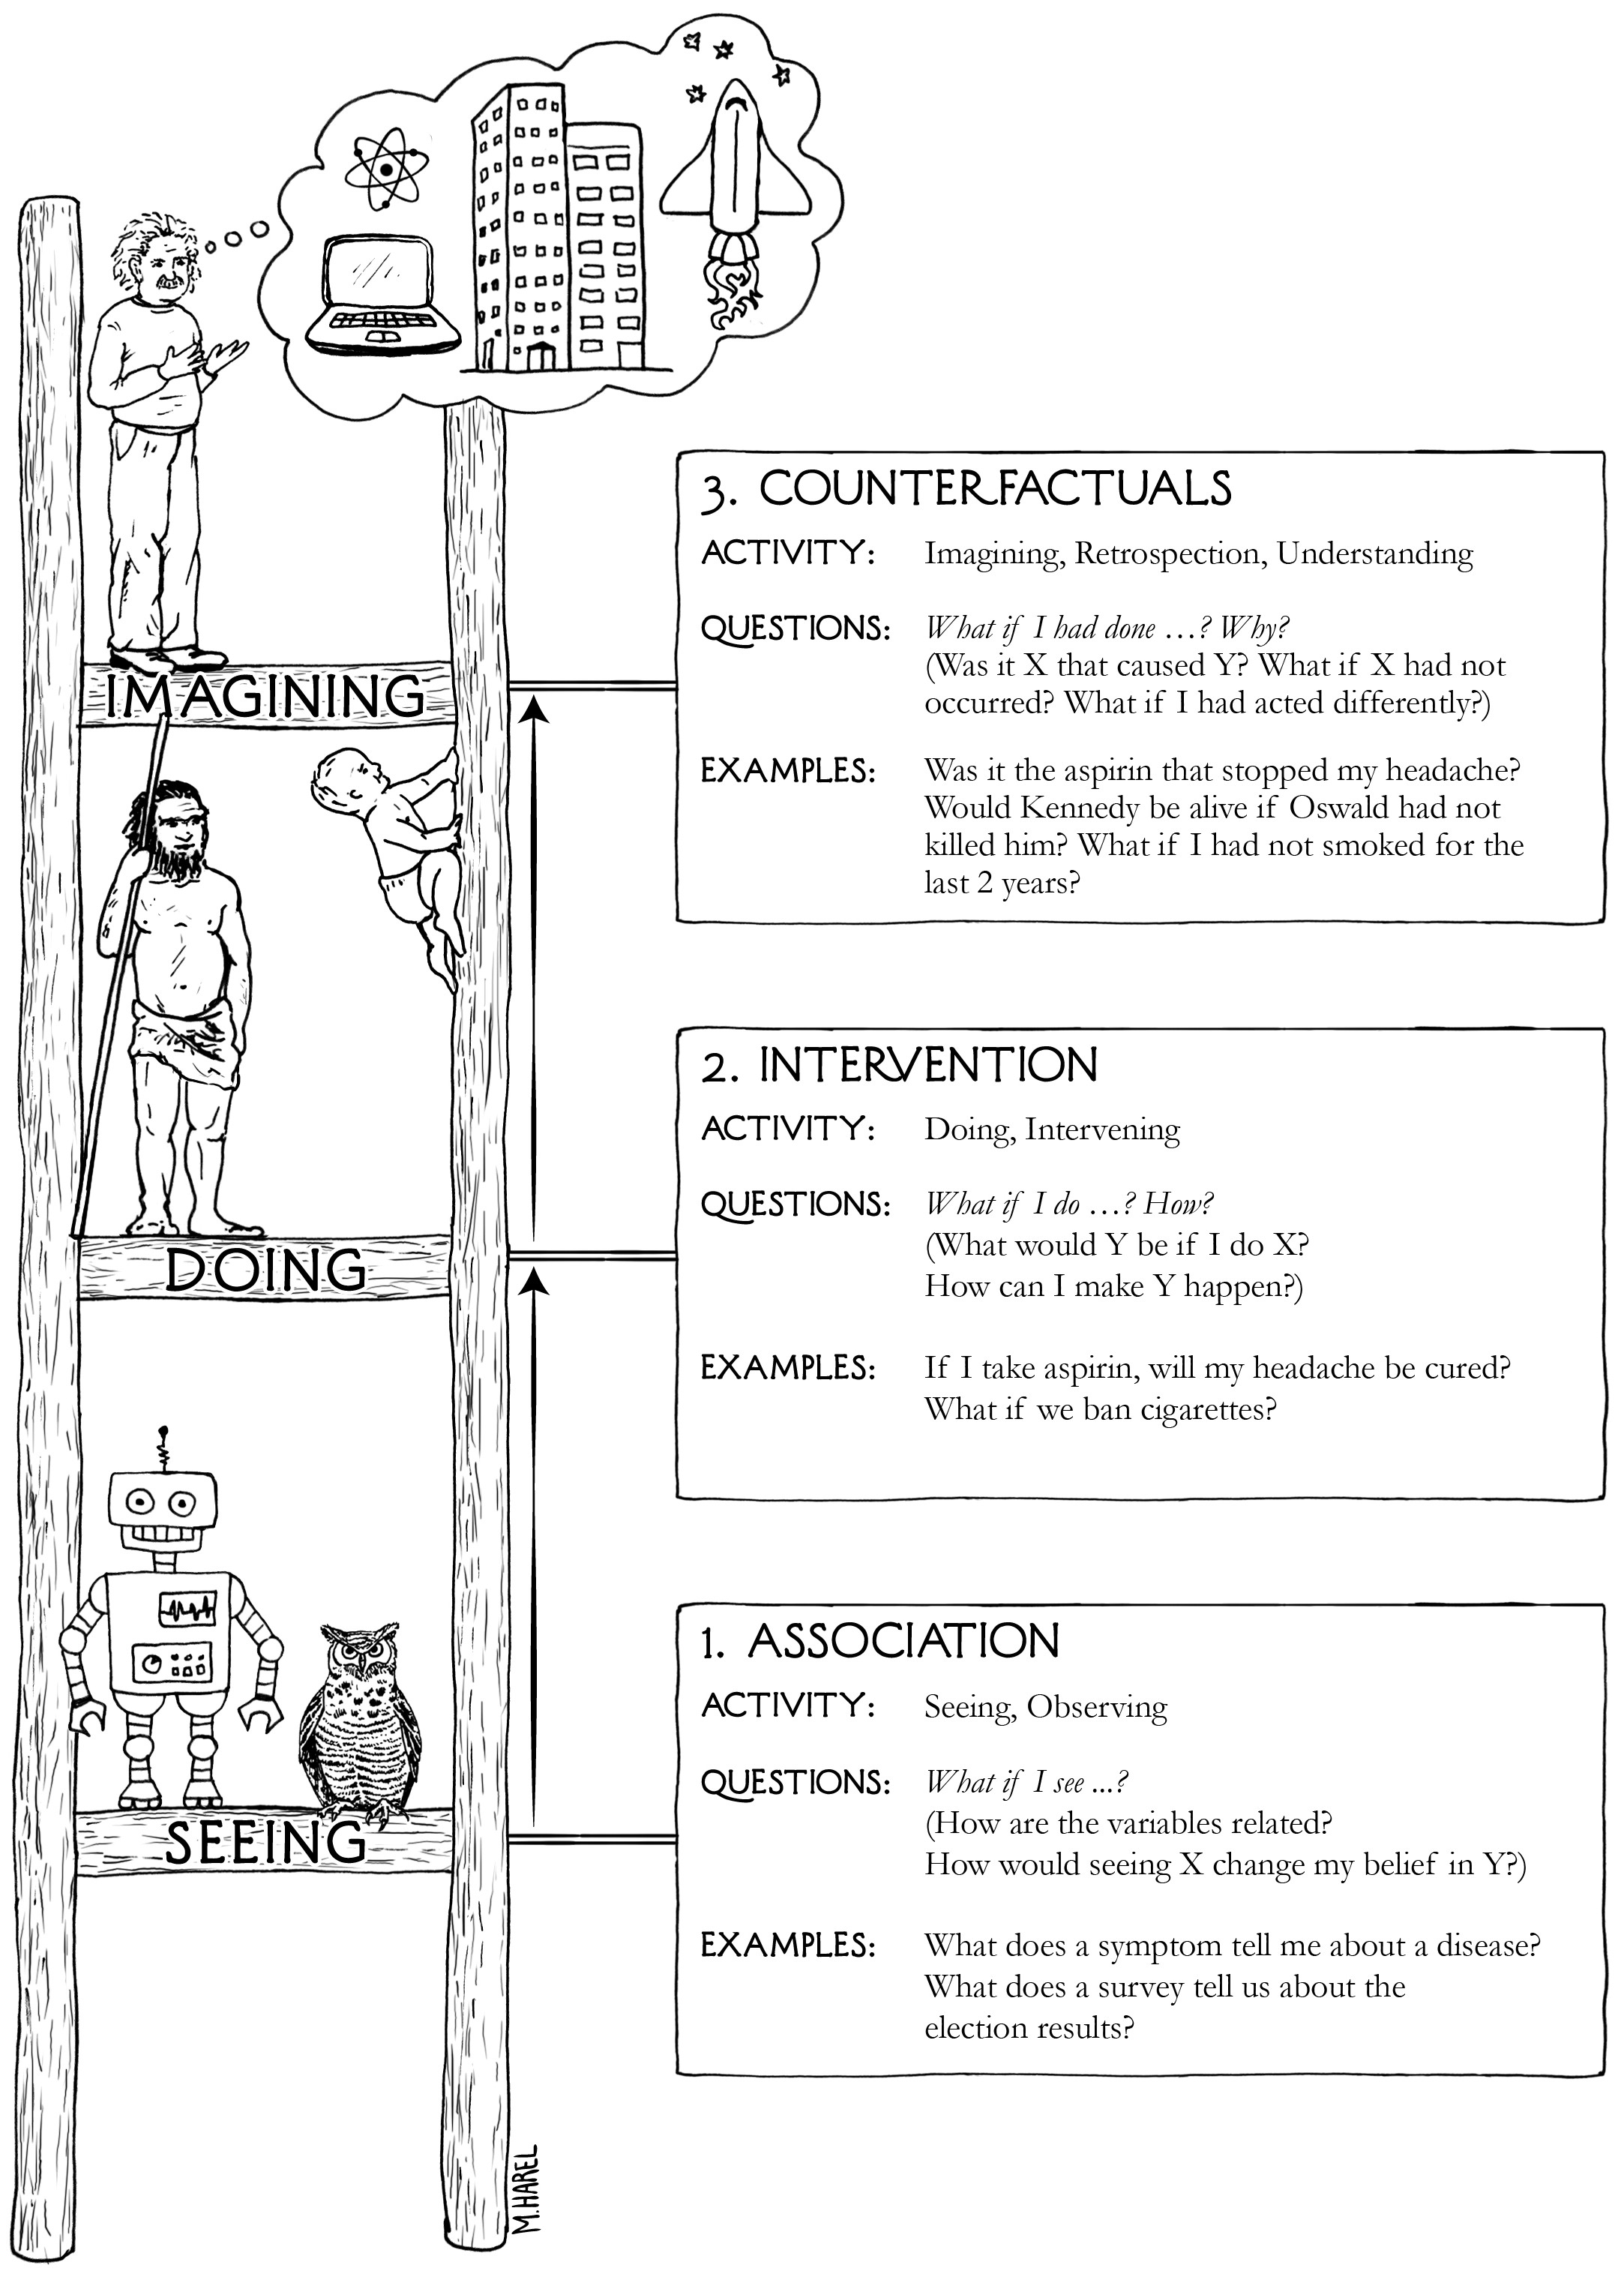
\includegraphics[width=0.45\textwidth]{ladder.jpg}};
    \draw[line width=1mm,fill=green,draw=green,->] (-4,2) -- node[below,sloped] {data-driven} (-4,-2);
    \draw[line width=1mm,fill=red,draw=red,->] (4,-2) -- node[below,sloped] {model-based} (4,2);
  \end{tikzpicture}
  \centerline{\tiny Image from Pearl \& Mackenzie, {\it The Book of Why}}
\end{frame}

\begin{frame}{Counterexample 2 (Dawid, 2002)}
\begin{example}[1/2]
  For parameter $\rho\in[0,1]$, consider the SCM $\C{M}_\rho$ with binary exogenous input variable $X \in \{0,1\}$, endogenous variable $Y \in \RN$, a single latent exogenous random variable $W = (W_1,W_2) \in \RN^2$ with
exogenous distribution 
  $$\begin{pmatrix} W_1 \\ W_2 \end{pmatrix}\sim\C{N}\left(\begin{pmatrix}0 \\ 0\end{pmatrix},\begin{pmatrix}1&\rho\\ \rho&1\end{pmatrix}\right)$$
and structural equation
  $$Y = W_1 (1 - X) + W_2 X.$$
  In a medical setting, this SCM could be used to model whether a patient was treated ($x$) and the corresponding outcome for that patient ($Y^{\doit(x)}$).
\end{example}
\end{frame}

\begin{frame}{Counterexample 2 (Dawid, 2002)}
\begin{example}[2/2]
  Suppose in the actual world, $x = 0$ and $Y^{\doit(x=0)} = y \in \RN$.
  Consider the counterfactual: {\it ``What would the outcome have been, had we assigned treatment to this patient?''}.

  Construct the twin SCM $\C{M}_{\rho}^{\twin}$.
  The counterfactual query then asks for $P_{M_{\rho}^\twin}((Y')^{\doit(x'=1)}=y'\mid Y^{\doit(x=0)}=y)$. One can calculate that
$$
  P_{M_{\rho}^\twin}\big((Y')^{\doit(x'=1)},Y^{\doit(x=0)}\big) = \C{N}\left(\begin{pmatrix}0\\ 0\end{pmatrix}, \begin{pmatrix} 1 & \rho \\ \rho & 1 \end{pmatrix}\right)
$$
  and hence $P_{M_{\rho}^\twin}((Y')^{\doit(x'=1)} \mid Y^{\doit(x=0)}=y) = \C{N}(\rho y,1-\rho^2)$. Note that the answer to the counterfactual query depends on a quantity $\rho$ that we cannot identify from the Markov kernel $P_{M_{\rho}}(Y\given \doit X)$, since this is independent of $\rho$. 
Indeed, SCMs $\C{M}_{\rho}$ and $\C{M}_{\rho'}$ with $\rho\neq\rho'$ are interventionally equivalent, but not counterfactually equivalent.
%If we obtain the SCM from a reduction, we find the one with $\rho = 1$.
\end{example}
  \textbf{Conclusion: counterfactuals cannot be learned from data alone!}
\end{frame}
